\documentclass[bachelor, och, coursework]{SCWorks}
% параметр - тип обучения - одно из значений:
%    spec     - специальность
%    bachelor - бакалавриат (по умолчанию)
%    master   - магистратура
% параметр - форма обучения - одно из значений:
%    och   - очное (по умолчанию)
%    zaoch - заочное
% параметр - тип работы - одно из значений:
%    referat    - реферат
%    coursework - курсовая работа (по умолчанию)
%    diploma    - дипломная работа
%    pract      - отчет по практике
% параметр - включение шрифта
%    times    - включение шрифта Times New Roman (если установлен)
%               по умолчанию выключен
\usepackage{subfigure}
\usepackage{tikz,pgfplots}
\pgfplotsset{compat=1.5}
\usepackage{float}

%\usepackage{titlesec}
\setcounter{secnumdepth}{4}
%\titleformat{\paragraph}
%{\normalfont\normalsize}{\theparagraph}{1em}{}
%\titlespacing*{\paragraph}
%{35.5pt}{3.25ex plus 1ex minus .2ex}{1.5ex plus .2ex}

\titleformat{\paragraph}[block]
{\hspace{1.25cm}\normalfont}
{\theparagraph}{1ex}{}
\titlespacing{\paragraph}
{0cm}{2ex plus 1ex minus .2ex}{.4ex plus.2ex}

% --------------------------------------------------------------------------%


\usepackage[T2A]{fontenc}
\usepackage[utf8]{inputenc}
\usepackage{graphicx}
\graphicspath{ {./images/} }
\usepackage{tempora}

\usepackage[sort,compress]{cite}
\usepackage{amsmath}
\usepackage{amssymb}
\usepackage{amsthm}
\usepackage{fancyvrb}
\usepackage{listings}
\usepackage{listingsutf8}
\usepackage{longtable}
\usepackage{array}
\usepackage[english,russian]{babel}

% \usepackage[colorlinks=true]{hyperref}
\usepackage{url}

\usepackage{underscore}
\usepackage{setspace}
\usepackage{indentfirst} 
\usepackage{mathtools}
\usepackage{amsfonts}
\usepackage{enumitem}
\usepackage{tikz}

\newcommand{\eqdef}{\stackrel {\rm def}{=}}
\newcommand{\specialcell}[2][c]{%
\begin{tabular}[#1]{@{}c@{}}#2\end{tabular}}

\renewcommand\theFancyVerbLine{\small\arabic{FancyVerbLine}}

\newtheorem{lem}{Лемма}

\begin{document}

% Кафедра (в родительном падеже)
\chair{теоретических основ компьютерной безопасности и криптографии}

% Тема работы
\title{Обнаружение объектов на изображении искусственными нейронными сетями}

% Курс
\course{2}

% Группа
\group{231}

% Факультет (в родительном падеже) (по умолчанию "факультета КНиИТ")
\department{факультета КНиИТ}

% Специальность/направление код - наименование
%\napravlenie{09.03.04 "--- Программная инженерия}
%\napravlenie{010500 "--- Математическое обеспечение и администрирование информационных систем}
%\napravlenie{230100 "--- Информатика и вычислительная техника}
%\napravlenie{231000 "--- Программная инженерия}
\napravlenie{100501 "--- Компьютерная безопасность}

% Для студентки. Для работы студента следующая команда не нужна.
% \studenttitle{Студентки}

% Фамилия, имя, отчество в родительном падеже
\author{Улитина Ивана Владимировича}

% Заведующий кафедрой
% \chtitle{} % степень, звание
% \chname{}

%Научный руководитель (для реферата преподаватель проверяющий работу)
\satitle{доцент} %должность, степень, звание
\saname{Слеповичев И. И.}

% Руководитель практики от организации (только для практики,
% для остальных типов работ не используется)
% \patitle{к.ф.-м.н.}
% \paname{С.~В.~Миронов}

% Семестр (только для практики, для остальных
% типов работ не используется)
%\term{8}

% Наименование практики (только для практики, для остальных
% типов работ не используется)
%\practtype{преддипломная}

% Продолжительность практики (количество недель) (только для практики,
% для остальных типов работ не используется)
%\duration{4}

% Даты начала и окончания практики (только для практики, для остальных
% типов работ не используется)
%\practStart{30.04.2019}
%\practFinish{27.05.2019}

% Год выполнения отчета
\date{2021}

\maketitle

% Включение нумерации рисунков, формул и таблиц по разделам
% (по умолчанию - нумерация сквозная)
% (допускается оба вида нумерации)
% \secNumbering

%-------------------------------------------------------------------------------------------

\tableofcontents

\intro

    В современном мире, в эпоху информационных технологий, с каждым годом увеличивается количество задач, которые могут быть решены с помощью компьютера. И чем сложнее компьютер становится, тем более серьезные проблемы становятся решаемыми. Однако были такие задачи, которые легко решались только человеческим разумом, за счет интуиции, а не вычислительной машины, так как лучше всего компьютером разрешались такие задачи, которые имели математическую составляющую, подход к которым осуществлялся с помощью определенного набора аксиом и правил. Совсем недавно, относительно появления компьютера, начала развиваться наука об искусственном интеллекте, которая открыла компьютерам возможность находить решения для таких проблем, которые раньше могли быть решены только человеком. Вследствие всего этого сейчас активно начала использоваться технология нейронных сетей, которая позволяет решать простые человеческие проблемы достаточно быстро, упрощая повседневную жизнь людей. В качестве примера таких задач можно привести: определение самого короткого маршрута из точки А в точку Б с учетом трафика в городе, перевод с одного языка на другой, автоматическое определение диагноза пациента при наборе симптомов, парковка машины с помощью искусственного интеллекта, сведение звука в музыкальных произведениях, классификация большого объема данных каких-либо форматов по различным нетривиальным или неоднозначным ключам, определение объектов на изображении, формирование прогноза погоды на основе некоторой метеорологической базе данных, предсказание курса ценных бумаг и многое другое.\\
    В данной работе будет рассматриваться задача обнаружения объектов на изображении посредством искусственных нейронных сетей, её примеры в реальной жизни, математическая составляющая её решения и анализ соответствующих этому решению инструментов.

\section{Концепция технологии}

    \subsection{Основные термины}
        Перед анализом математической составляющей нейросети, работающей с конкретной задачей (в данном случае "--- с анализом изображений на предмет обнаружения объектов) стоит ввести ряд терминов, которые являются фундаментом понимания работы нейросетей.\\
        Каждый отдельный элемент информации, включаемый в представление о каком-либо анализируемом объекте, называется \textbf{признаком}. Большая часть задач искусственного интеллекта решается в два этапа: корректный подбор признаков, а затем их передача алгоритму машинного обучения. В качестве примера можно взять задачу идентификации объекта по звуку речи. В ней полезным признаком является речевой тракт или же голосовой диапазон. Он
        позволяет с большой точностью определить, является ли говорящий объект мужчиной, женщиной или
        ребенком.
        Но далеко не во задачах можно сразу понять, какие признаки стоит выделять: для этого достаточно рассмотреть ситуацию, в которой необходимо написать программу обнаружения автомобилей на фотографиях. Известно, что у автомобилей есть колеса, вследствии чего можно в качестве одного из признаков выбрать наличие колеса. Однако нельзя сказать, что описание колеса на уровне пикселей легкая задача.
        Колесо характеризуется простой геометрической формой, но его распознавание на изображении
        нередко бывает осложнено различными факторами, такими как отбрасывание теней, наличие щитка для защиты колеса от грязи, объекты на переднем плане, которые могут закрывать часть колеса, и т. д.

        В качестве решений подобной задачи рассматривают использование машинного обучения не только как способа нахождения отображения представления на результат, но и для определения самого представления. Такой подход к реализации машинного обучения называется \textbf{обучением представлений}. С помощью этих представлений, которые являются результатом обучения, получается более точно определить объект на изображении, чем с помощью представлений, созданных вручную. В качестве характерного преимущества подобных реализаций стоит отметить быструю адаптацию ИИ к новым задачам с учетом минимального вмешательства человека в изменение структуры конкретной нейросети. 

        Важную роль в алгоритме обучения представлений является понятие \textbf{автокодировщика} - совокупность функции кодирования (которая преобразует входные данные в удобное для решения задачи представление) и функции декодирования, являющейся обратной по смыслу к предыдущей функции. Обучение автокодировщиков устроено таким образом, что при каждой последующей итерации, в ходе которой происходит кодирование и декодирование некоторой информации, каждое новое представление характеризуется всё большим количеством полезных свойств при наименьшей потери обрабатываемой информации.

        Сутью моделирования алгоритма обучения признаков или же самого признака является получение различных \textbf{факторов вариативности}. Фактор вариативности в контексте машинного обучения "--- концепция, помогающая получить смысл из данных той характеристики об изучаемом объекте, которая может иметь большое количество различных значений, то есть обладающая высокой вариативностью. Например, в случае анализа изображения машины такие абстракции как её положение, цвет, яркость солнца и его высота над горизонтом являются факторами вариативности, а в случае анализа изображения лица человека факторами вариативности будут являтся его цвет, положение и цвет глаз, их расстояние друг от друга, положение и форма губ, и так далее. Однако большое количество факторов вариативности, получаемых в ходе проектирования признаков или иным способом, следует отбросить в силу их влияния на все данные, доступные анализу в процессе обучения нейросети (например, форма губ человека при изучении изображения лица зависит от угла зрения и может быть распознана алгоритмом машинного обучения некорректно).

        Проблему получения представления решает \textbf{глубокое обучение}, которое осуществляет их получение путем их выражения через более простые представления, а формирование последних, в свою очередь, реализуется через ещё более простые представления, и так далее.

        \begin{figure}[H]
            \centering
            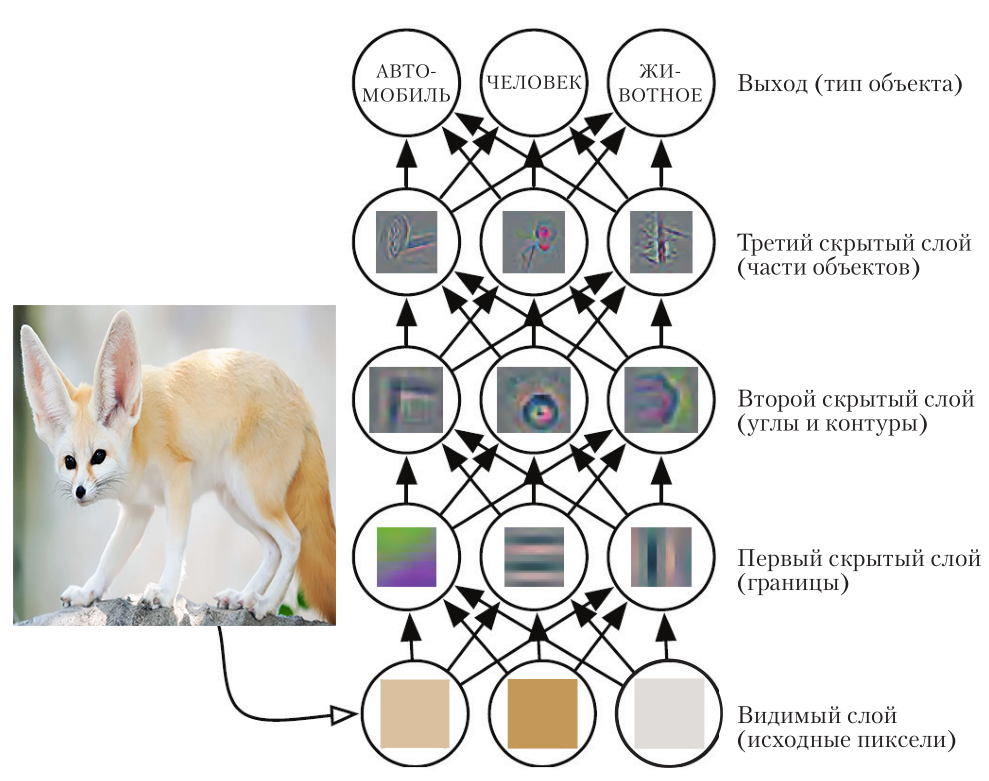
\includegraphics[width=0.9\textwidth]{pic/1.png}
            \caption{Пример модели глубокого обучения "--- определение объекта на изображении}
            \label{fig:img1}
        \end{figure}

        Определение объекта на изображении, представленном в виде набора значений пикселей, трудно решаема при использовании функции отображения множества пикселей в распознаваемый объект. Использование в рассматриваемом случае глубокого обучения на порядок упрощает задачу за счёт разбиения исходного набора пикселей на некоторое количество более простых вложенных отображений, описываемых отдельным слоем модели для каждого. Входные данные в виде изображения представляют из себя входной, или \textbf{видимый слой} (англ. ''input layer'') (слой называется видимым, так как содержит открытые данные, включащие в себя доступные для изучения переменные). После видимого слоя идет совокупность \textbf{скрытых слоев} (англ. ''hidden layer''), представляющих из себя слои математических функций, каждый из которых предназначен для вычисления значения, являющегося специфичным для ожидаемого результата (их количество напрямую определяет глубину обучения, так как каждый из них извлекает из анализируемого изображения некоторые признаки, и чем больше таких слоев, тем более абстрактные признаки будут получены из исходных данных). Скрытыми они называются в связи с тем, что осуществляют вычисления и генерируют данные, не являющиеся изначальными. Модель самостоятельно определяет пользу каждой из абстракций при конструировании связей в наблюдаемых данных. Завершающим глубокое обучение и определяющим (в данном случае) объект на изображении является \textbf{выходной слой} (англ. ''output layer''). На рисунке 1 в составе модели глубокого обучения представлены 3 скрытых слоя, а также слой входных данных и слой выходных данных. При анализе изображения, в силу доступности информации об исходных пикселях (определяемых входным слоем), первый скрытый слой определяет границы совокупностей пикселей с помощью сравнения последних по признаку яркости соседних пикселей. Имея характеристики границ множеств пикселей, полученные в результате действия первого скрытого слоя, второй определяет углы и контуры, представляемые в виде набора границ. На основании этих данных третий скрытый слой осуществляет распознавание частей конкретных объектов на изображении, представленных в виде совокупностей углов и контуров отдельного вида. А последний, выходной слой определяет объекты на изображении по информации о частях этих объектов. 

    \subsection{Математическая составляющая нейросети}
        Структура нейросети представляет из себя совокупность деятельности нескольких математических дисциплин, среди которых выделяют: линейную алгебру, теорию вероятностей и теорию графов. В связи с этим, наиболее популярно представление нейронной сети в виде перцептрона. Перцептрон (или же в некоторых источниках персептрон) "--- это математическая модель, целью которой является интерпретация деятельности человеческого мозга посредством вышеупомянутых областей математики. Другое определение перцептрона "--- это ориентированный граф, вершины которого описывают входные, скрытые и выходные слои модели машинного обучения (структура которого была описана пунктом выше), связанные друг с другом с помощью ребер, каждое из которых обладает собственным весом, которое может быть как статично, так и дифференцируемо в зависимости от определения поведения нейронной сети при решении конкретной задачи (однако стоит отметить, что, несмотря на возможность изображения перцептрона в виде графа, никаких практических преимуществ в этом нет, так как большая часть реализаций перцептрона не подразумевает использование алгоритмов теории графов). Также, перцептрон можно описать как математическую функцию, возвращающую множество выходных данных при принятии в качестве аргументов множества входных данных.
        
        % ИЗОБРАЖЕНИЕ ПЕРЦЕПТРОНА С РАЗЛИЧНЫМИ ПОМЕТКАМИ
        \begin{figure}[H]
            \centering
            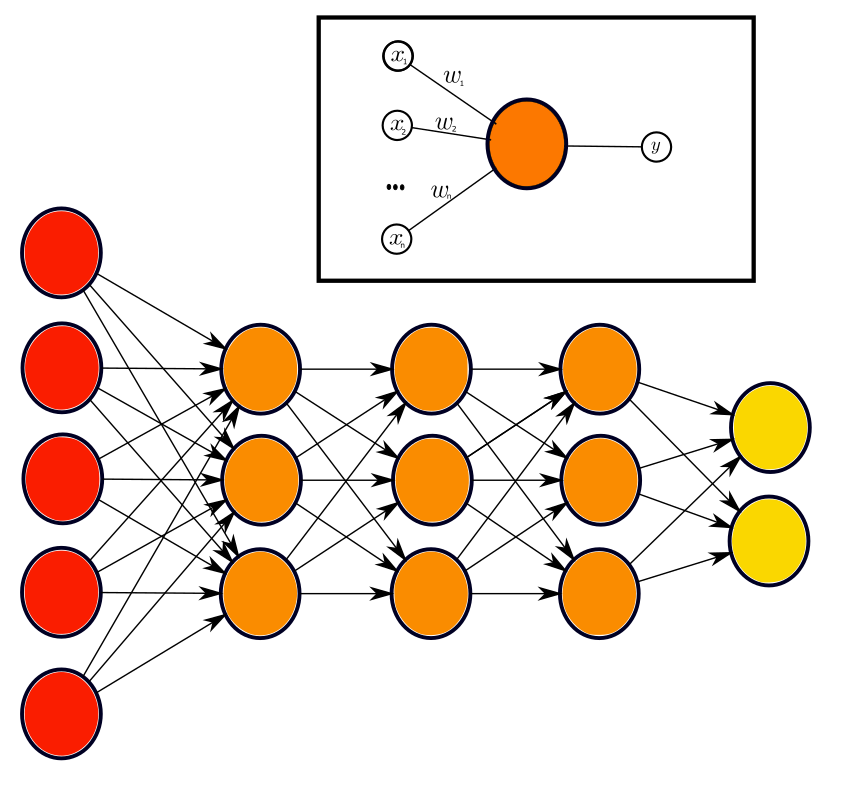
\includegraphics[width=0.9\textwidth]{pic/perceptron.png}
            \caption{Многослойный перцептрон и устройство нейрона}
            \label{fig:img2}
        \end{figure}
        
        На рис. 2 изображен многослойный перцептрон, состоящий из искусственных нейронов, соединенных друг с другом синапсом (или же дугой/стрелкой). Каждый синапс имеет собственный вес, определяющий влияние входных данных нейрона на его состояние, а также на значение, которое этот нейрон возвращает, характеризуемое различными формулами в зависимости от вида нейрона.
        
        Наиболее популярно представление нейрона как преобразователя одного входного элемента в один выходной элемент в некоторый дискретный момент времени с шагом $\tau$. Например, пусть входной сигнал "--- $x$, а $\alpha$ "--- характеристика (или их набор) рассматриваемого нейрона $f(x, \alpha)$, тогда можно выделить несколько видов нейронов:
        \newpage
        \begin{enumerate}
            \item Пороговый нейрон (где $x \geq 0$ и $\alpha > 0$)
                \begin{equation*}
                    f(x) = 
                     \begin{cases}
                       0 &\text{если $x < \alpha$}\\
                       1 &\text{если $x \geq \alpha$}
                     \end{cases}
                \end{equation*}    
            \item (при $-\infty < x < \infty, \alpha > 0$) \[f(x) = \frac{x}{\alpha + | x |}\]
            \item (при $-\infty < x < \infty, \alpha > 0$) \[f(x) = th\frac{x}{\alpha}\]
            \item Многопараметрические нейроны: (при $\alpha_2 > 0, \hspace{5pt} -\infty < x, \hspace{5pt} \alpha_{1, 3} < \infty$)
                \[f(x) = \frac{\alpha_1 \cdot x + | x | \cdot x}{\alpha_2 + \alpha_3 \cdot | x | + x^2}\]
            \item (при $\alpha_3 > 0, \hspace{5pt} -\infty < x, \hspace{5pt} \alpha_{1, 2, 4, 5} < \infty$)
                \[f(x) = \frac{\alpha_1 \cdot x + \alpha_2 \cdot x^2 + x^3}{\alpha_3 + \alpha_4 \cdot | x | + \alpha_5 \cdot x^2 + | x |^3}\]
        \end{enumerate}

        В частности, для обнаружения объектов на изображении, используется \textbf{сверточная} нейронная сеть "--- специальная разновидность нейросети, обрабатывающая данные с сеточной топологией и характерузующая технологию компьютерного зрения. Название этой сети напрямую связано с алгебраической линейной операцией свертки, сутью которой является получение функции из двух других функций. Сверточная сеть предполагает использование операции свертки вместо общей операции умножения на матрицу в по крайней мере одном слое.
        % \[S = \sum_{i = 1}^n x_i w_i \]
        
        % Существует несколько разновидностей перцептрона:
        % \begin{enumerate}
        %     \item 
        % \end{enumerate}

\section{Реализация технологии}

    \subsection{Инструменты}
            
    \subsection{Препроцессинг (формирование датасета)}
            
    \subsection{Обучение}
        

\section{Применение технологии}

    Распознавание визуальных образов является одной из самых важных
    деталей большинства систем управления и анализа информации, а также
    автоматизированных систем. Задачи, которые связаны с определением предметов,
    описываемых конечным перечнем особых свойств и признаков, имеют место в некоторых 
    отраслях деятельности машинного обучения, такие как робототехника, мониторинг, анализ
    визуальных данных, исследования искусственного интеллекта и т.д. Обработка алгоритмами и
    классификация изображений активно используются в кибербезопасности, в системах контроля и
    управления доступом, в системах видеонаблюдения, виртуальной и дополненной
    реальности и информационных поисковых системах. В настоящий момент в
    производстве активно применяются алгоритмы распознавания рукописного текста,
    номеров транспортных средств, отпечатков пальцев, человеческих лиц или иных средств аутентификации человека, имеющие огромный спрос при реализации интерфейсов программ, систем безопасности и иных прикладных целей.

    \subsection{Задачи мониторинга}
        
        В этом пункте будет рассматриваться применение искусственных сверточных нейронных сетей, выполняющих задачу обнаружения объектов на изображении, для определения разнообразных видов и моделей самолётов, которые находятся на территории аэропорта. Результат работы над конкретной проблемой будет представлять из себя информацию, используемую в различных задачах мониторинга взлётно-посадочных полос (например, определение количества самолетов конкретного вида).

    \subsection{Задачи анализа визуальных данных}
            
    \subsection{Реализация интерфейса}

\conclusion

\end{document}
